\begin{figure}
 \centering
 \begin{subfigure}[b]{\textwidth}
  \begin{columns}
  \begin{column}{0.10\textwidth}
   \caption{}%
   \label{fig:cheek_cell}
  \end{column}
  \begin{column}{0.75\textwidth}
    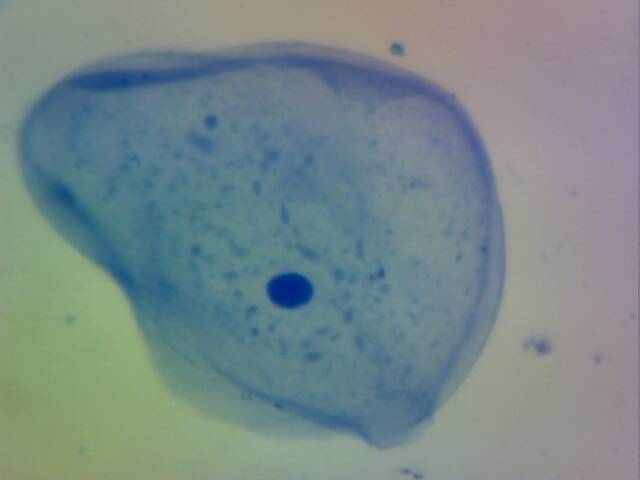
\includegraphics[width=\textwidth]{img/cheek_cell}
  \end{column}
  \begin{column}{0.05\textwidth}
    \cite{clare_and_ben_2017}
  \end{column}
  \end{columns}
 \end{subfigure}\\
 \begin{subfigure}[b]{\textwidth}
  \begin{columns}
  \begin{column}{0.10\textwidth}
   \caption{}%
   \label{fig:ant}
  \end{column}
  \begin{column}{0.75\textwidth}
    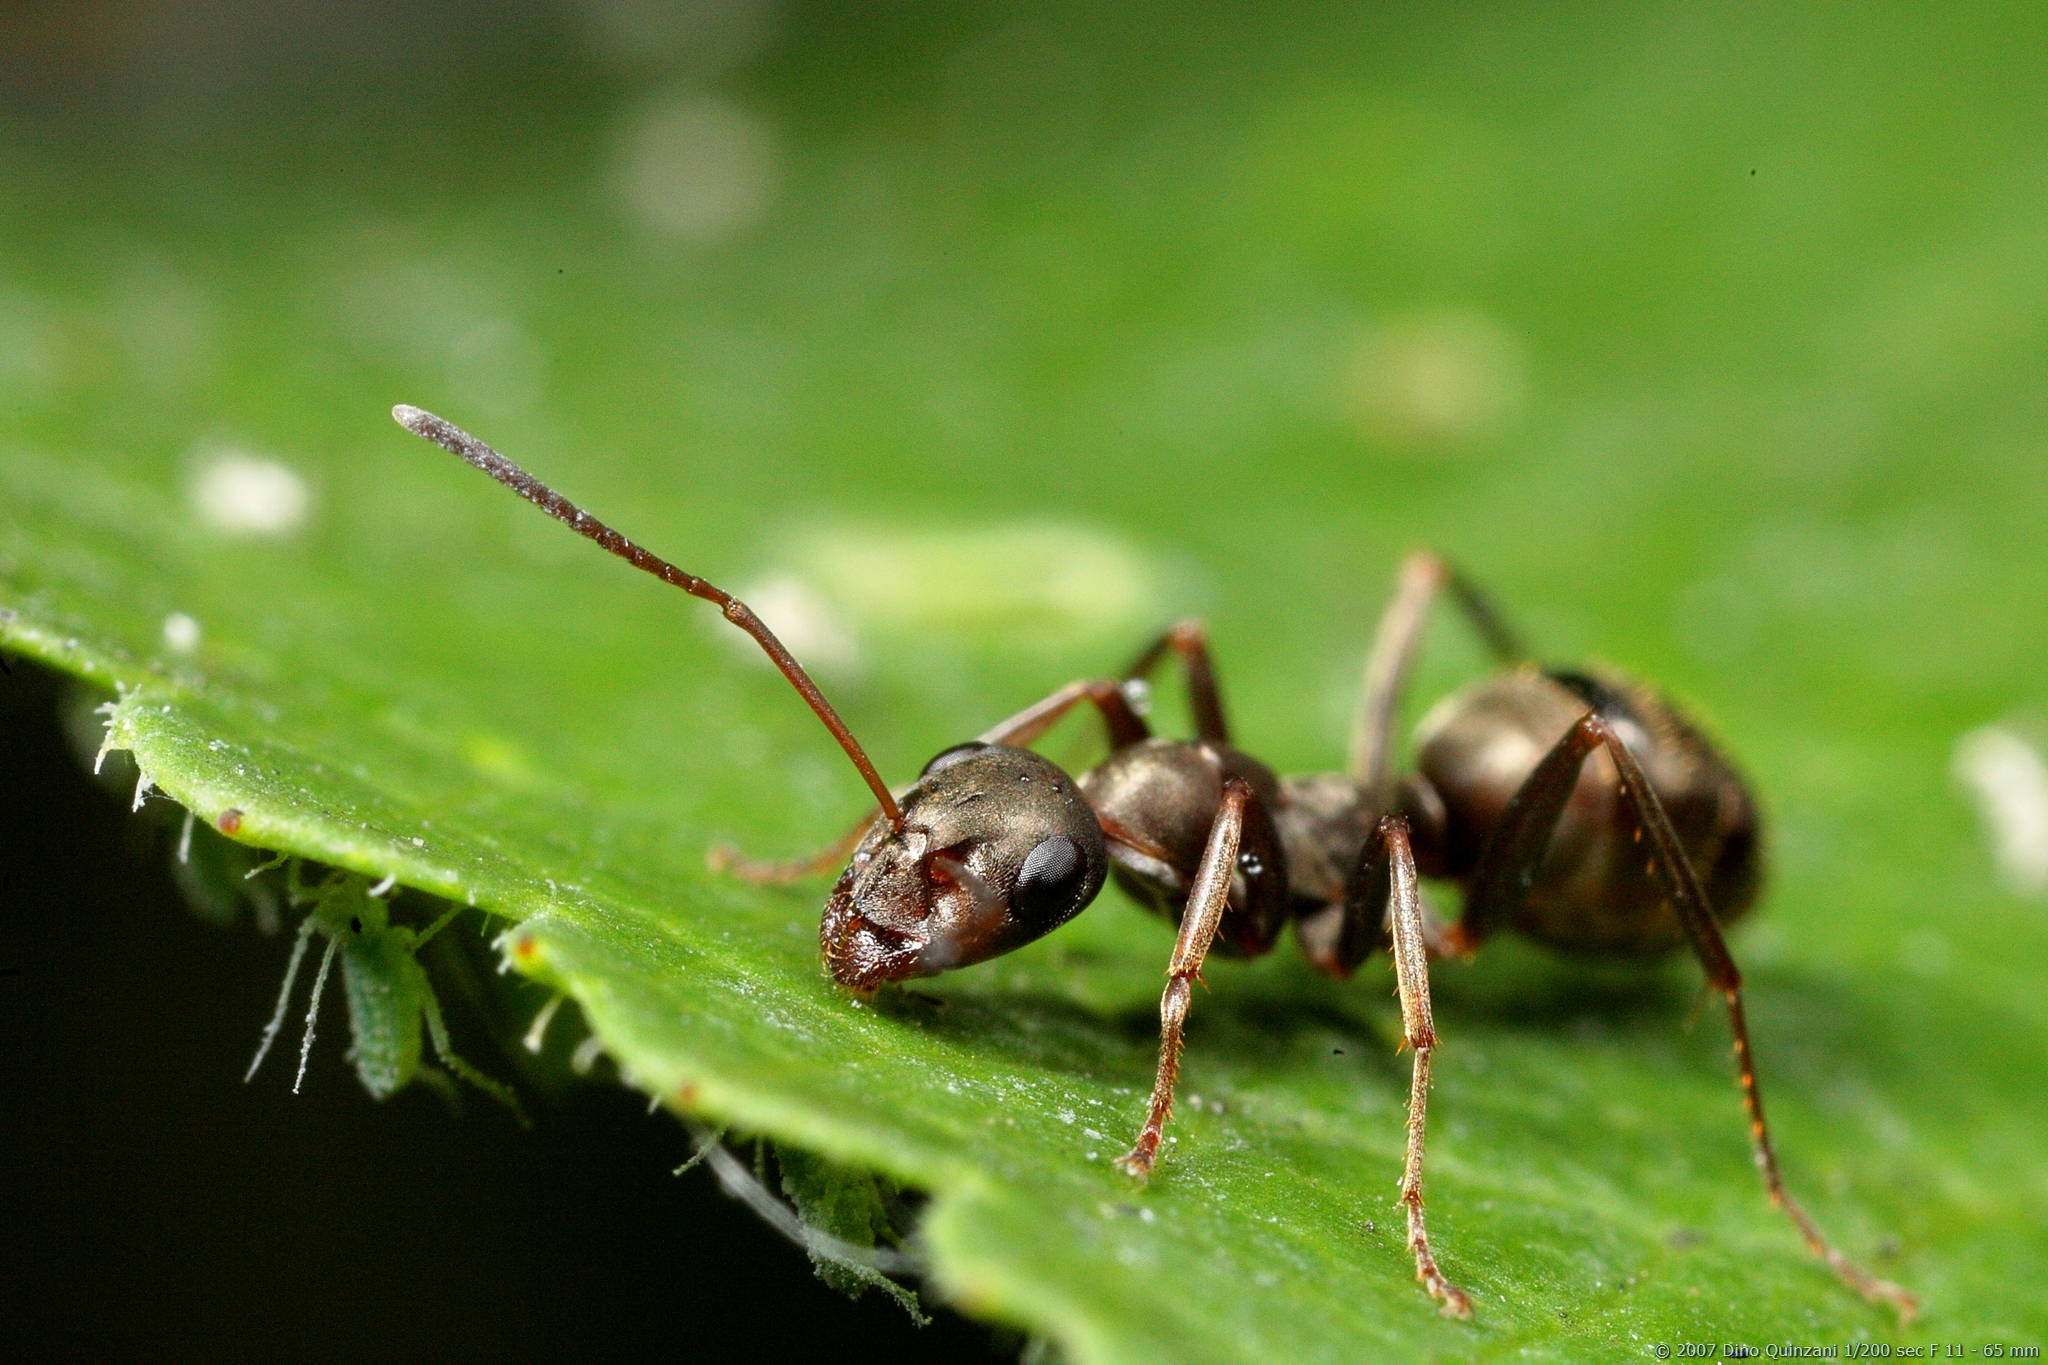
\includegraphics[width=\textwidth]{img/ant}
  \end{column}
  \begin{column}{0.05\textwidth}
    \cite{quinzani_2008}
  \end{column}
  \end{columns}
 \end{subfigure}\\
 \begin{subfigure}[b]{\textwidth}
  \begin{columns}
  \begin{column}{0.10\textwidth}
   \caption{}%
   \label{fig:ant_bridge}
  \end{column}
  \begin{column}{0.75\textwidth}
    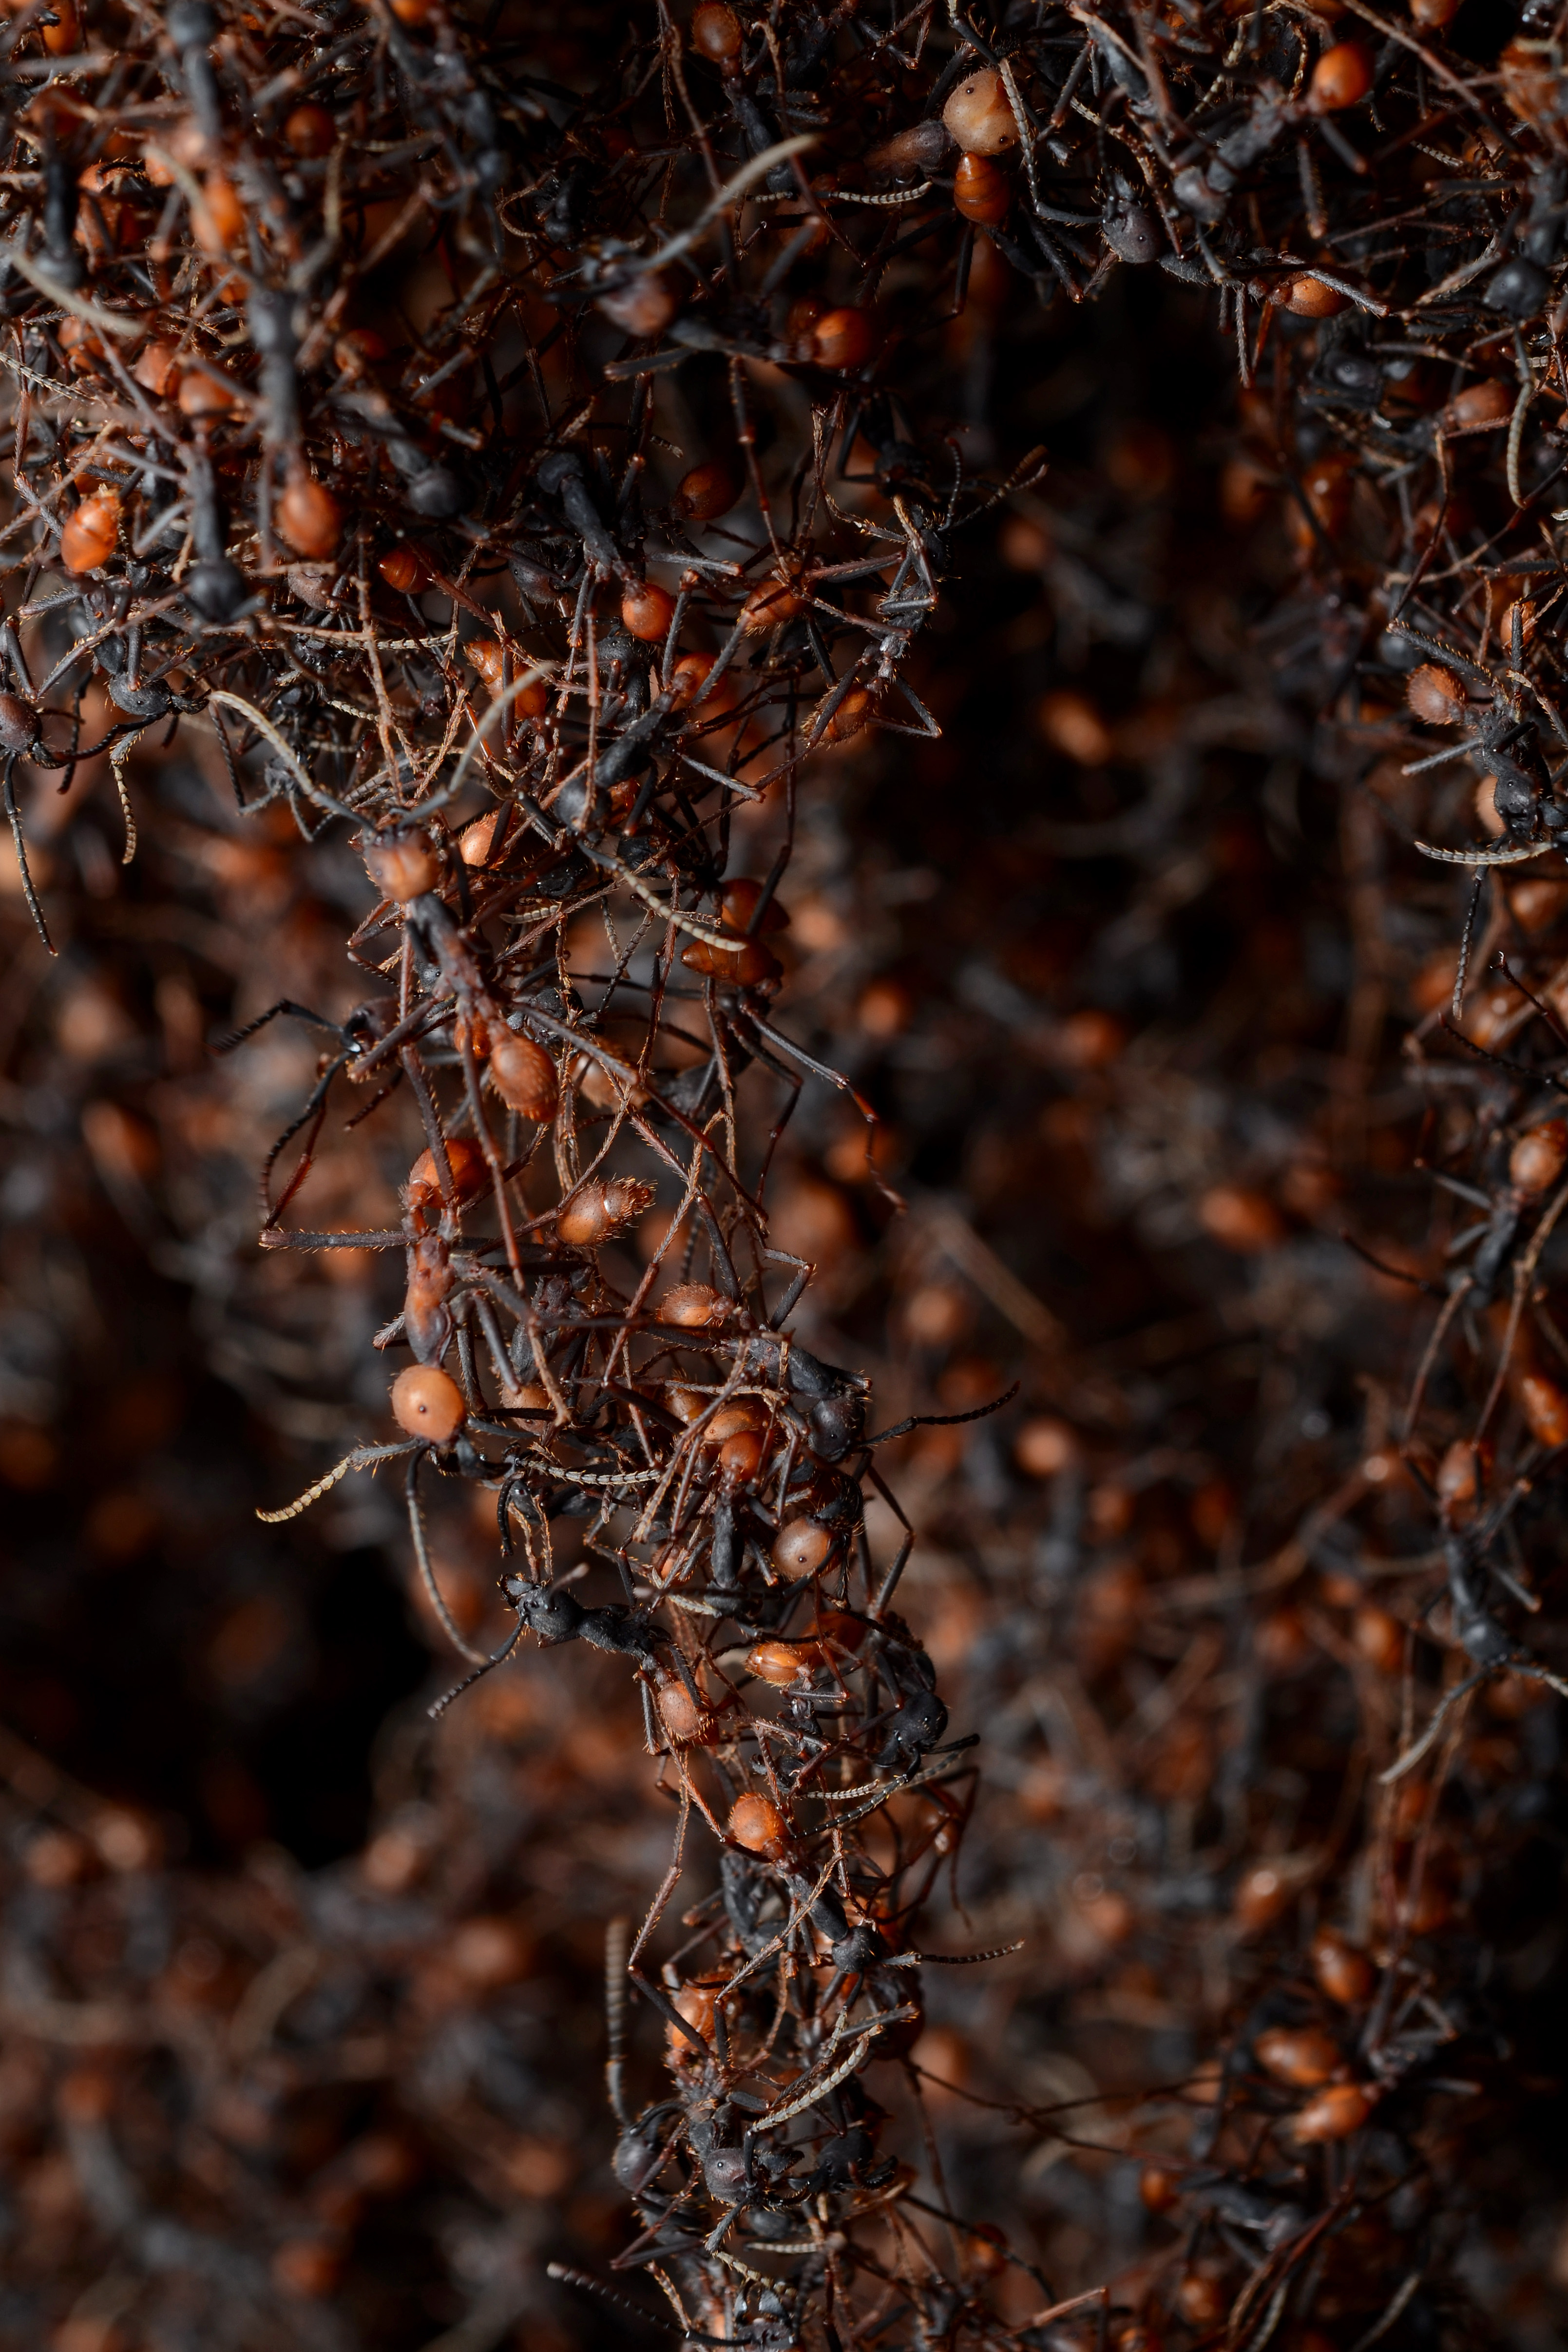
\includegraphics[angle=270,width=\textwidth]{img/ant_bridge}
  \end{column}
  \begin{column}{0.05\textwidth}
    \cite{gallice_2011}
  \end{column}
  \end{columns}
 \end{subfigure}
 \caption{
 Example of nested fraternal transitions of individuality where cells (\ref{fig:cheek_cell}) unite into multicellular ants (\ref{fig:ant}), which in turn unite into ant colonies (\ref{fig:ant_bridge}).
 }
 \label{fig:fraternal}
\end{figure}
